\documentclass[a4paper, 11pt]{article}

%%% SST LAB PROTOCOLL PREAMBLE
%%% 2019
%%%%%%%%%%%%%%%%%%%%%%%%%%%%%%%


%%% PACKAGES
%%%%%%%%%%%%%%%%%%%%%%%%%%%

\usepackage[ngerman]{babel}

\usepackage[utf8]{inputenc}
\usepackage{amsmath}
\usepackage{pgfplots}
\usepackage{tikz}
\usepackage[many]{tcolorbox}
\usepackage{graphicx}
\graphicspath{ {./graphics/} }
\usepackage{pdfpages}
\usepackage{dashrule}
\usepackage{float}
\usepackage{siunitx}
\usepackage{booktabs}
\usepackage[version=4]{mhchem}

%%% DOCUMENT GEOMETRY
%%%%%%%%%%%%%%%%%%%%%%%%%%%

\usepackage{geometry}
\geometry{
 a4paper,
 total={0.6180339887498948\paperwidth,0.6180339887498948\paperheight},
 top = 0.1458980337503154\paperheight,
 bottom = 0.1458980337503154\paperheight
 }
\setlength{\jot}{0.013155617496424828\paperheight}
\linespread{1.1458980337503154}

\setlength{\parskip}{0.013155617496424828\paperheight} % paragraph spacing


%%% COLORS
%%%%%%%%%%%%%%%%%%%%%%%%%%%

\definecolor{red1}{HTML}{f38181}
\definecolor{yellow1}{HTML}{fce38a}
\definecolor{green1}{HTML}{95e1d3}
\definecolor{blue1}{HTML}{66bfbf}
\definecolor{hsblue}{HTML}{00b1db}
\definecolor{hsgrey}{HTML}{afafaf}

%%% CONSTANTS
%%%%%%%%%%%%%%%%%%%%%%%%%%%
\newlength{\smallvert}
\setlength{\smallvert}{0.0131556\paperheight}


%%% COMMANDS
%%%%%%%%%%%%%%%%%%%%%%%%%%%

% differential d
\newcommand*\dif{\mathop{}\!\mathrm{d}}

% horizontal line
\newcommand{\holine}[1]{
  	\begin{center}
	  	\noindent{\color{hsgrey}\hdashrule[0ex]{#1}{1pt}{3mm}}\\%[0.0131556\paperheight]
  	\end{center}
}

% mini section
\newcommand{\minisec}[1]{ \noindent\underline{\textit {#1} } \\}

% quick function plot
\newcommand{\plotfun}[3]{
  \vspace{0.021286\paperheight}
  \begin{center}
    \begin{tikzpicture}
      \begin{axis}[
        axis x line=center,
        axis y line=center,
        ]
        \addplot[draw=red1][domain=#2:#3]{#1};
      \end{axis}
    \end{tikzpicture}
  \end{center}
}

% box for notes
\newcommand{\notebox}[1]{

\tcbset{colback=white,colframe=red1!100!black,title=Note!,width=0.618\paperwidth,arc=0pt}

 \begin{center}
  \begin{tcolorbox}[]
   #1 
  \end{tcolorbox}
 
 \end{center} 
 
}

% box for equation
\newcommand{\eqbox}[2]{
	
	\tcbset{colback=white,colframe=hsblue!100!black,title=,width=#2,arc=0pt}
	
	\begin{center}
		\begin{tcolorbox}[ams align*]
				#1
		\end{tcolorbox}
		
	\end{center} 
	
}

% END OF PREAMBLE
%%%%%%%%%%%%%%%%%%%%%%%%%%%%%%%%%%%%%

% for logic expressions
\colorlet{highcolor}{black}
\colorlet{lowcolor}{black}
\newcommand{\HIGH}{
  {\color{highcolor}{HIGH}}
}
\newcommand{\LOW}{
  {\color{lowcolor}{LOW}}
}


\begin{document}

% 1
%%%%%%%%%%%%%%%%%%%%%%%%%%%%%%%%%%%%%
  
\includepdf{./titlepage/titlepage1.pdf}
  \clearpage
  \setcounter{page}{1}
%%%%%%%%%%%%%%%%%%%%%%%%%%%%%%%%%%%%%

\section{Schmitt-Trigger}
\begin{figure}[t]
  \begin{center}
    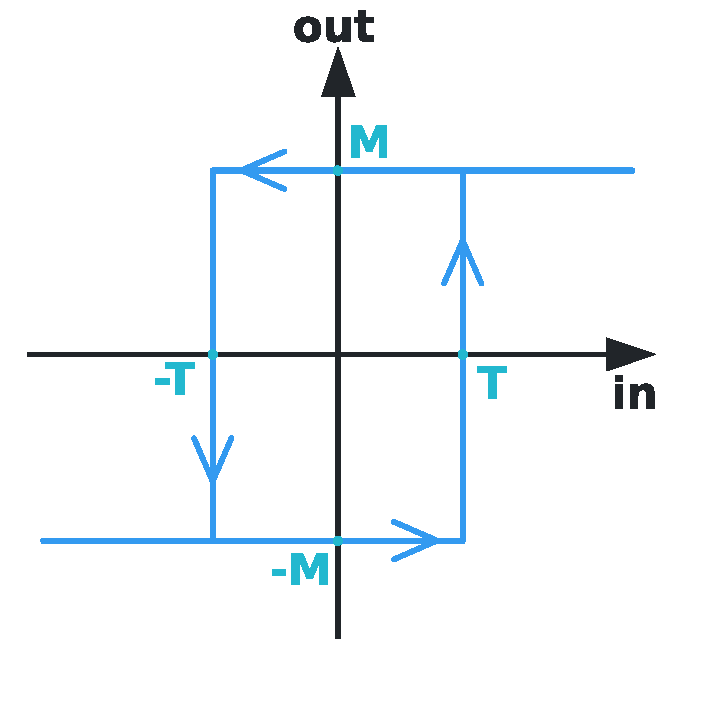
\includegraphics[width=0.382\textwidth]{VBA/1/Hysteresis}
  \end{center}
  \caption{Vereinfachte Kennlinie eines (nichtinvertierenden) Schmitt-Triggers (Quelle: Wikipedia)}
\end{figure}
Ein Schmitt-Trigger ist eine Art des Komparators, dessen Ein-Ausgangs-Kennlinie
einer Hysterese unterliegt, welche durch zwei Schwellenwerte charakterisiert ist.


Gerät die (analoge) Eingangsspannung über den oberen Schwellwert \textit{T} läuft die
Ausgangsspannung des Triggers auf ihren maximalen positiven Wert \textit{M} (Sättigung). In diesem
Fall bewirkt die weitere Erhöhung der Eingangsspannung keine Veränderung der
Ausgangsspannung. Erst wenn der Eingangsspannungswert auf den unteren
Schwellwert \textit{$-T$} abfällt, ändert sich die Ausgangsspannung auf den
maximal negativen Wert \textit{$-M$}. Analog gilt hier, dass sich erst bei
Überschreitung der oberen Schwelle die Ausgangsspannung wieder ändert. 

Ein Schmitt-Trigger kann beispielsweise mithilfe eines positiv-rückgekoppelten
Operationsverstärkers realisiert werden.


\section{Monostabiler Multivibrator (Monoflop)}
Ein monostabiler Multivibrator (auch monost. Kippstufe, Monoflop) generiert bei Triggerung einen Ausgangsimpuls definierter Länge.

\emph{Nachtriggerbare} Monoflops haben die Eigenschaft, während des aktiven
Ausgangszustandes durch ein erneutes Eingangssignal neugestartet zu werden,
wodurch sich die Ausgangsimpulsdauer verlängert. 

Monoflops können z.B. verwendet werden, um Tasterprellen zu unterdrücken,
indem sie durch den ersten Prellimpuls ausgelöst werden und dann für eine
bestimmte Zeit im aktiven Zustand bleiben, in welchem keine weiteren
Prellimpulse eine Ausgangsänderung hervorrufen können.

\begin{figure}[]
  \begin{center}
    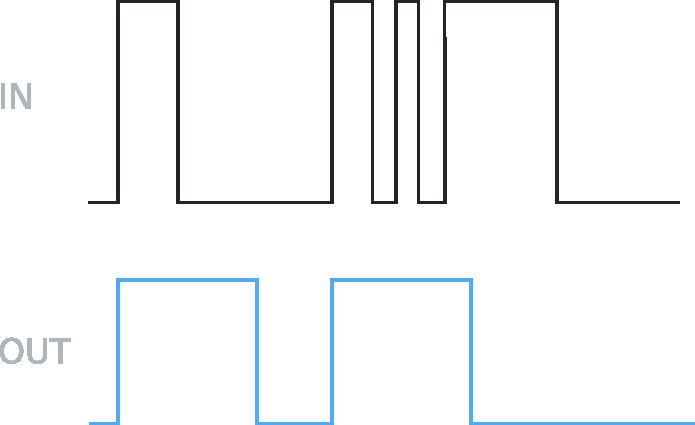
\includegraphics[width=0.382\textwidth]{VBA/2/monoop}
  \end{center}
  \caption{Beispielhafter Signalverlauf eines Monoflops}
\end{figure}

\section{Funktionsweise des Monoflops}
\begin{figure}[h]
  \begin{center}
    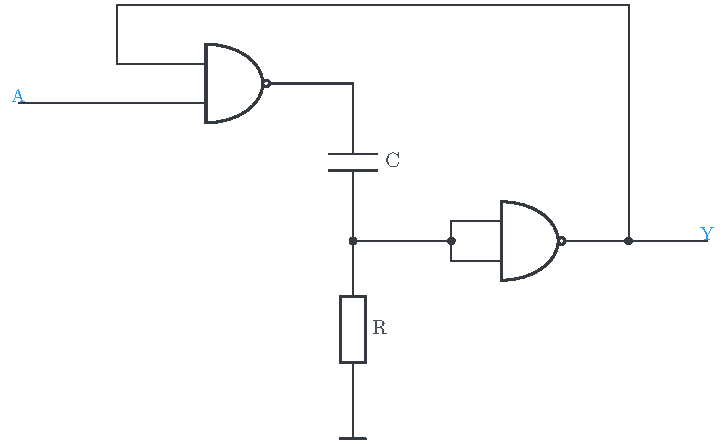
\includegraphics[width=0.618\textwidth]{VBA/3/monoflop}
  \end{center}
  \caption{Monoflopschaltung mit zwei NAND-Gattern}
  \label{fig:monoflop2}
\end{figure}

Die Schaltung aus Abbildung \ref{fig:monoflop2} ist eine Monostabile Kippstufe
mit zwei NAND-Gattern und einer RC-Kombination. Das zweite NAND-Gatter stellt
durch die Verbindung beider Eingangsleitungen einen einfachen Invertierer dar.

Im Ruhezustand (stabiler Zustand) der Schaltung ist Eingang A \HIGH und der
Ausgang des zweiten NAND-Gatters (Y) \HIGH. Durch die Rückkopplung des Ausganges Y wird der Ausgang des ersten
NANDs \LOW und es finden keine Pegeländerungen statt.

Findet nun ein \HIGH \to \LOW Übergang an A statt, wird der Ausgang des ersten
NANDs \HIGH, wodurch der Kondensator C geladen wird. Im Umschaltzeitpunkt des
ersten Gatters liegt dessen volle Ausgangsspannung am Widerstand R an, da der
Kondensator ungeladen ist und über ihn somit keine Spannung abfällt.

Die Spannung über dem Widerstand entspricht der Eingangsspannung des Inverters,
wodurch die Ausgangsspannung zu \LOW wechselt und der Kondensator weiter geladen wird.

Steigt die Spannung über dem Kondensator, so sinkt die Spannung über dem
Widerstand. Ist der Kondensator ausreichend geladen, um die Spannung über dem
Widerstand so verringert zu haben, dass die Eingangsschwelle des Inverters für
die logische Zuordnung (z.B. $2\,\si{\volt}$) unterschritten wird, wechselt der
Ausgang Y auf \HIGH. 

Ändert sich A nun wieder auf \HIGH entlädt sich der Kondensator, da Y=\HIGH und
A=\HIGH und somit der Ausgang des ersten NANDs \LOW ist. Durch den Entladestrom
des Kondensators ist der Spannungsabfall über dem Widerstand negativ in Bezug
auf Masse, weshalb sich der Eingangspegel des Inverters (\LOW) nicht ändert und
Y \HIGH bleibt.

Insgesamt ergibt sich also bei einem Eingangsimpuls ein Ausgangsimpuls, dessen Länge von der
Kondensatorladezeit abhängt.

Für die korrekte Funktion der Schaltung muss darauf geachtet werden, dass die
Länge des Eingangsimpulses deutlich länger ist als die des gewünschten
Ausgangsimpulses, um zu gewährleisten, dass der sich Kondensator ausreichend lädt/entlädt.
Bei zu frühem Wechsel des Eingangssignals auf \LOW bzw. \HIGH kann es daher
vorkommen, dass sich die Ausgangsimpulszeit verändert.

Um die negative Eingangsspannung am Gattereingang zu vermeiden, kann eine Diode
parallel zum Widerstand geschaltet werden. Weiterhin sollte zur Sicherstellung
des Ruhezustandes Eingang A mit einem Pull-Up-Widerstand versehen werden. Die
angepasste Schaltung ist in Abbildung \ref{fig:monoflop3} zu sehen.

\begin{figure}[]
  \begin{center}
    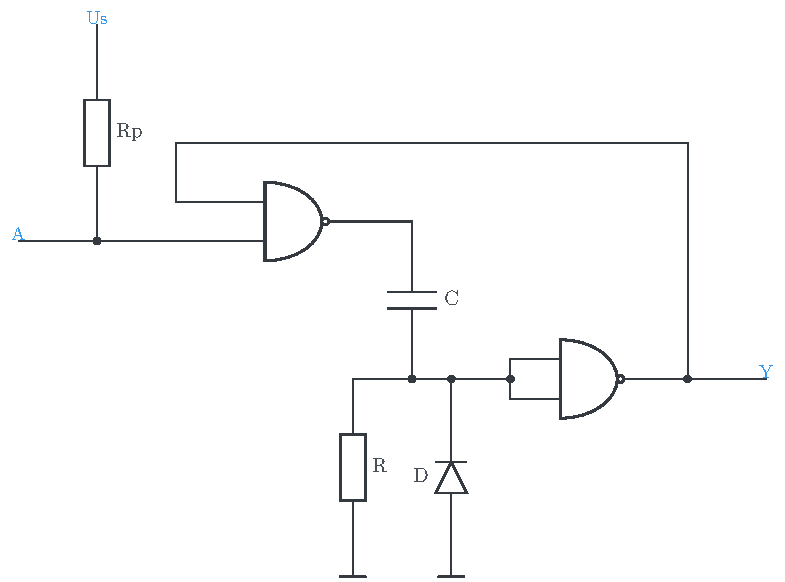
\includegraphics[width=0.618\textwidth]{VBA/3/monoflop2}
  \end{center}
  \caption{Verbesserte Monoflopschaltung}
  \label{fig:monoflop3}
\end{figure}


\section{Aufbau astabiler Multivibratoren}
\begin{figure}[h]
  \begin{center}
    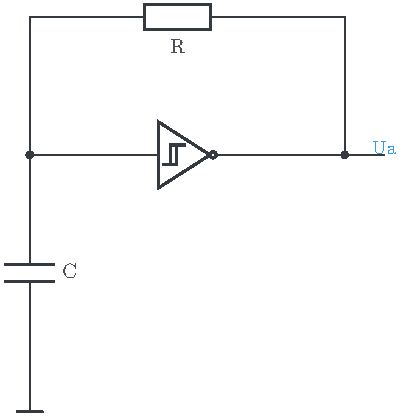
\includegraphics[height=0.382\textwidth]{VBA/4/astabil_schmitt}
  \end{center}
  \caption{Mutlivibratorschaltung mit Schmitt-Trigger}
  \label{fig:astable1}
\end{figure}

Astabile Multivibratoren besitzen keinen stabilen Ausgangszustand, weshalb sie
sich zur Taktgenerierung eignen. Abbildung \ref{fig:astable1} zeigt ein
Beispiel eines astabilen Multivibrators mit einem invertierenden Schmitt-Trigger
und einer RC-Kombination. Da es keinen stabilen Zustand gibt, sollte man zur Analyse einen
der Zustände an den Ausgängen der logischen Gatter annehmen, da diese nur 0 oder
$U_{\mathrm{S}}$ sein können. Ist zum Beispiel der Ausgang des Triggers
\HIGH, lädt sich der Kondensator $C$ über den Widerstand $R$ auf (unter der
Annahme, dass der Strom in/aus Gattereingänge/n vernachlässigbar ist). Erreicht
die Spannung über dem Kondensator (gegen Masse) den oberen Eingangsschwellwert
des Schmitt-Triggers, dann schaltet der Triggerausgang auf \LOW (invertierend).
Der Kondensator entlädt sich nun über $R$ bis die untere
Trigger-Eingangsschwelle erreicht ist und der Ausgang wieder zu \HIGH wird.

Abbildung \ref{fig:astable2} zeigt eine weitere Realisierungsmöglichkeit einer
astabilen Multivibratorschaltung mit zwei Invertern.

\begin{figure}[h]
  \begin{center}
    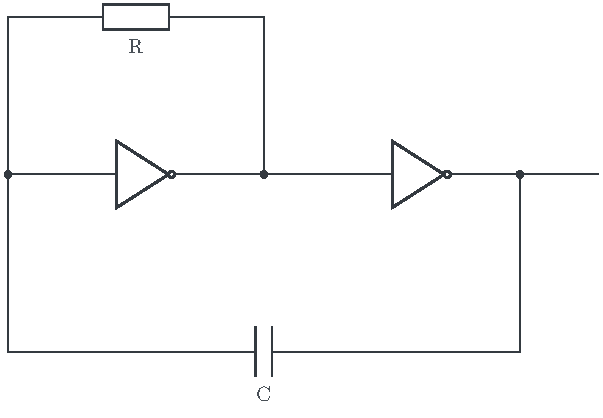
\includegraphics[width=0.618\textwidth]{VBA/4/astabil}
  \end{center}
  \caption{Weitere Möglichkeit einer astabilen Multivibratorschaltung}
  \label{fig:astable2}
\end{figure}



\section{Mono- und astabile Multivibratoren mit dem NE555}

\section{TTL-Definitionen}

\section{Statischer und dynamischer Störabstand}

\section{Lastfaktor bei Gatter-Zusammenschaltung}

\section{Eingangskennlinie eines 7400-Gatters}

\section{Open-Collector-Ausgang}

\section{Schaltkreisfamilien und deren Eigenschaften}

\section{Zusammenschaltung von Gattern unterschiedlicher Familie}

\end{document}
